\documentclass[11pt,a4paper]{article}

% CONFIGURACION
\usepackage[spanish]{babel}
\usepackage{amsmath,amssymb}
\usepackage{graphicx}
\usepackage{booktabs}
\usepackage{geometry}
\usepackage{float}
\usepackage{xcolor}
\usepackage{hyperref}

\geometry{margin=2.5cm}
\graphicspath{{outputs/graficos/}}
\setlength{\parindent}{0pt}
\setlength{\parskip}{0.5em}

\hypersetup{
    colorlinks=true,
    linkcolor=black,
    urlcolor=blue
}

\begin{document}

% PORTADA
\begin{titlepage}
\centering
\vspace*{2cm}

{\Large Universidad Yachay Tech\par}
\vspace{0.5cm}
{\large Maestría en Ciencia de Datos\par}
{\large Fundamentos de Inteligencia Artificial\par}

\vspace{2.5cm}

{\Huge\bfseries Actividad 5\par}
\vspace{0.5cm}

{\LARGE Clasificación supervisada mediante
K-Nearest Neighbors\par}

\vspace{0.8cm}
{\large Selección de hiperparámetros y
evaluación sobre Wine Recognition\par}

\vfill

{\large Autor: Mat. Héctor Alexander Román Potosí\par}

\vspace{1cm}

{\large Octubre de 2026\par}

\end{titlepage}

% RESUMEN
\begin{abstract}
Se implementó un clasificador de aprendizaje
supervisado basado en K-Nearest Neighbors (KNN)
para identificar tres clases de vinos mediante
trece características químicas.

Se emplearon 178 observaciones del conjunto Wine
Recognition, una división estratificada del 80\%
para entrenamiento y 20\% para prueba, y validación
cruzada estratificada de cinco particiones.

La búsqueda de hiperparámetros evaluó valores
de $K$ entre 1 y 60. El mejor valor observado
fue $K=29$, con una exactitud media de validación
de 97.88\%.

En la evaluación final se obtuvo una exactitud
de 97.22\%, correspondiente a 35 predicciones
correctas de 36.

\textbf{Palabras clave:} aprendizaje supervisado,
KNN, clasificación multiclase, validación cruzada,
selección de hiperparámetros.
\end{abstract}

\section{Introducción}

El aprendizaje supervisado permite construir modelos
predictivos utilizando observaciones cuyas etiquetas
son conocidas.

En problemas de clasificación, la variable objetivo
pertenece a un conjunto discreto de categorías.

El algoritmo K-Nearest Neighbors clasifica una nueva
observación utilizando las etiquetas de sus
$K$ vecinos más cercanos, de acuerdo con una
medida de distancia.

El objetivo de este estudio es seleccionar y
justificar el número de vecinos y evaluar el
desempeño del clasificador sobre observaciones
independientes del entrenamiento.

\section{Fundamentos matemáticos}

\subsection{Representación de los datos}

Se dispone de una matriz de características:

\begin{equation}
X \in \mathbb{R}^{178 \times 13}
\end{equation}

y un vector de etiquetas:

\begin{equation}
y \in \{0,1,2\}^{178}.
\end{equation}

El problema consiste en construir una función:

\begin{equation}
f:\mathbb{R}^{13}\rightarrow\{0,1,2\}.
\end{equation}

\subsection{Estandarización}

Debido a las diferencias de escala entre las
características, se utiliza StandardScaler:

\begin{equation}
z_{ij}=\frac{x_{ij}-\mu_j}{\sigma_j},
\end{equation}

donde $\mu_j$ y $\sigma_j$ representan,
respectivamente, la media y la desviación
estándar de la característica $j$ calculadas
sobre los datos de ajuste correspondientes.

\subsection{Distancia euclidiana}

La distancia entre dos observaciones
estandarizadas es:

\begin{equation}
d(z_i,z)=
\sqrt{\sum_{j=1}^{13}(z_{ij}-z_j)^2}.
\end{equation}

\subsection{Regla de clasificación}

Sea $\mathcal{N}_K(z)$ el conjunto de los
$K$ vecinos más cercanos a la observación $z$.

La clase predicha se obtiene mediante votación:

\begin{equation}
\hat y(z)=
\underset{c\in\{0,1,2\}}{\arg\max}
\sum_{i\in\mathcal{N}_K(z)}
\mathbf{1}(y_i=c).
\end{equation}

\section{Metodología}

\subsection{Conjunto de datos}

Se utilizó Wine Recognition, disponible mediante
Scikit-learn y procedente del repositorio UCI
Machine Learning.

El conjunto contiene 178 observaciones,
13 características numéricas y tres clases.

\begin{table}[H]
\centering
\caption{Distribución de las clases}
\begin{tabular}{lrr}
\toprule
Clase & Observaciones & Porcentaje \\
\midrule
0 & 59 & 33.15\% \\
1 & 71 & 39.89\% \\
2 & 48 & 26.97\% \\
\midrule
Total & 178 & 100\% \\
\bottomrule
\end{tabular}
\end{table}

No se identificaron valores faltantes ni
registros completamente duplicados.

\begin{figure}[H]
\centering
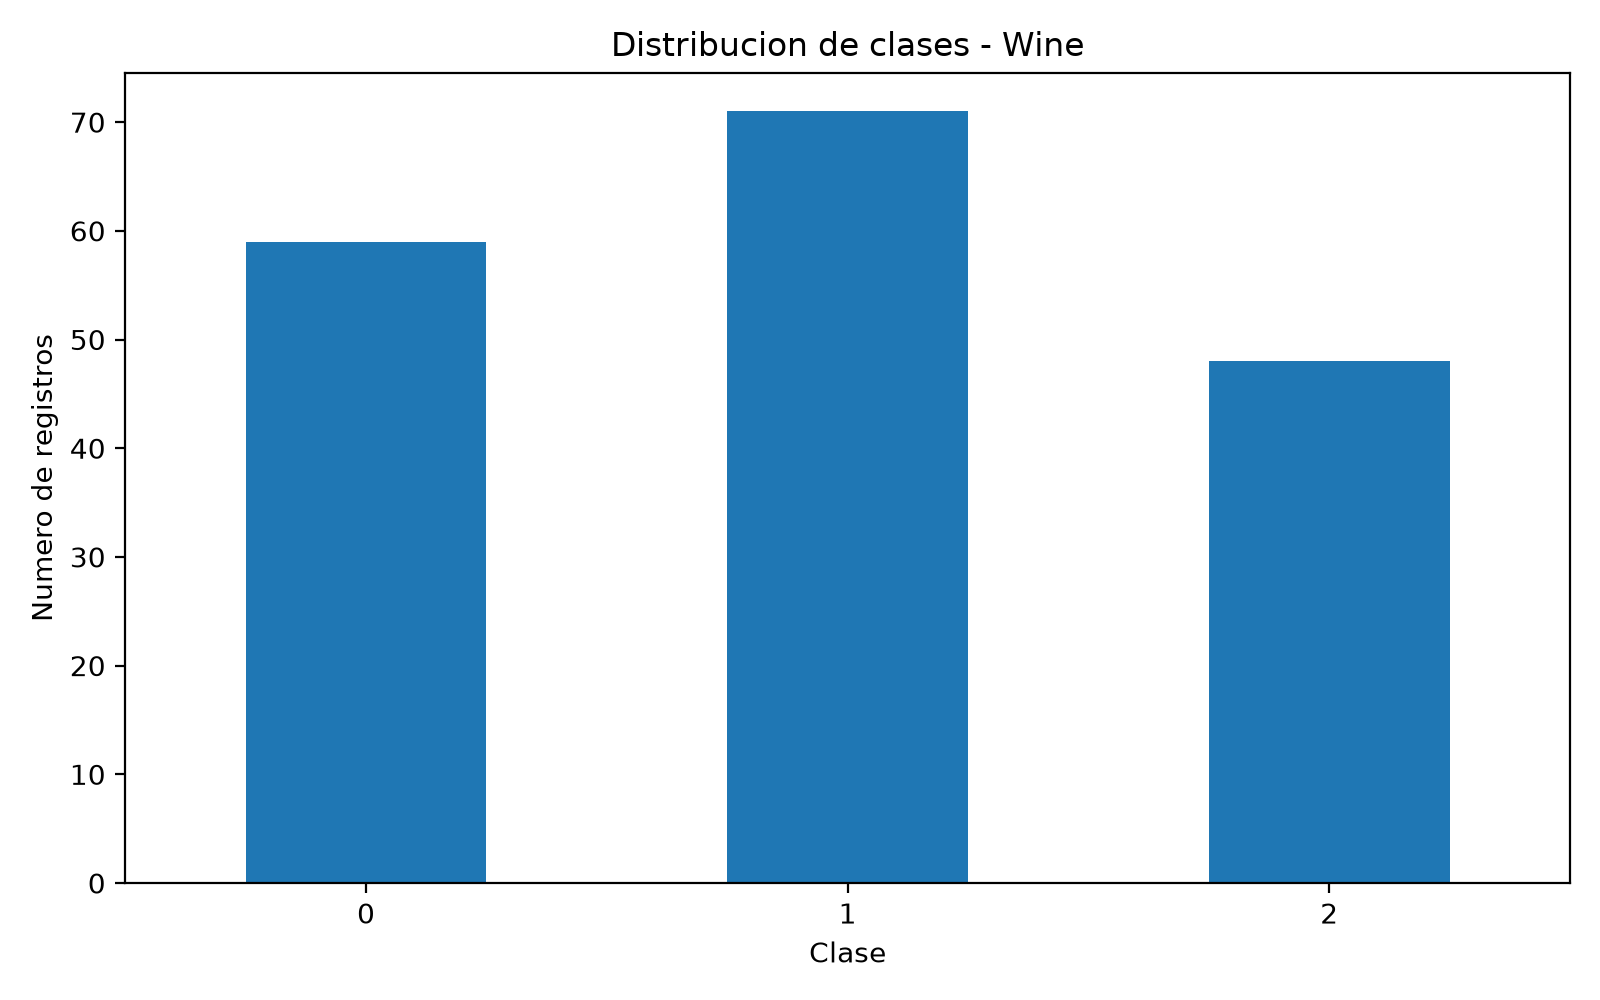
\includegraphics[
width=0.75\textwidth,
height=0.27\textheight,
keepaspectratio
]{distribucion_clases.png}
\caption{Distribución de las tres clases.}
\end{figure}

\subsection{Análisis exploratorio}

La representación de flavanoides e intensidad
de color muestra regiones donde las clases
se separan y otras donde se superponen.

\begin{figure}[H]
\centering
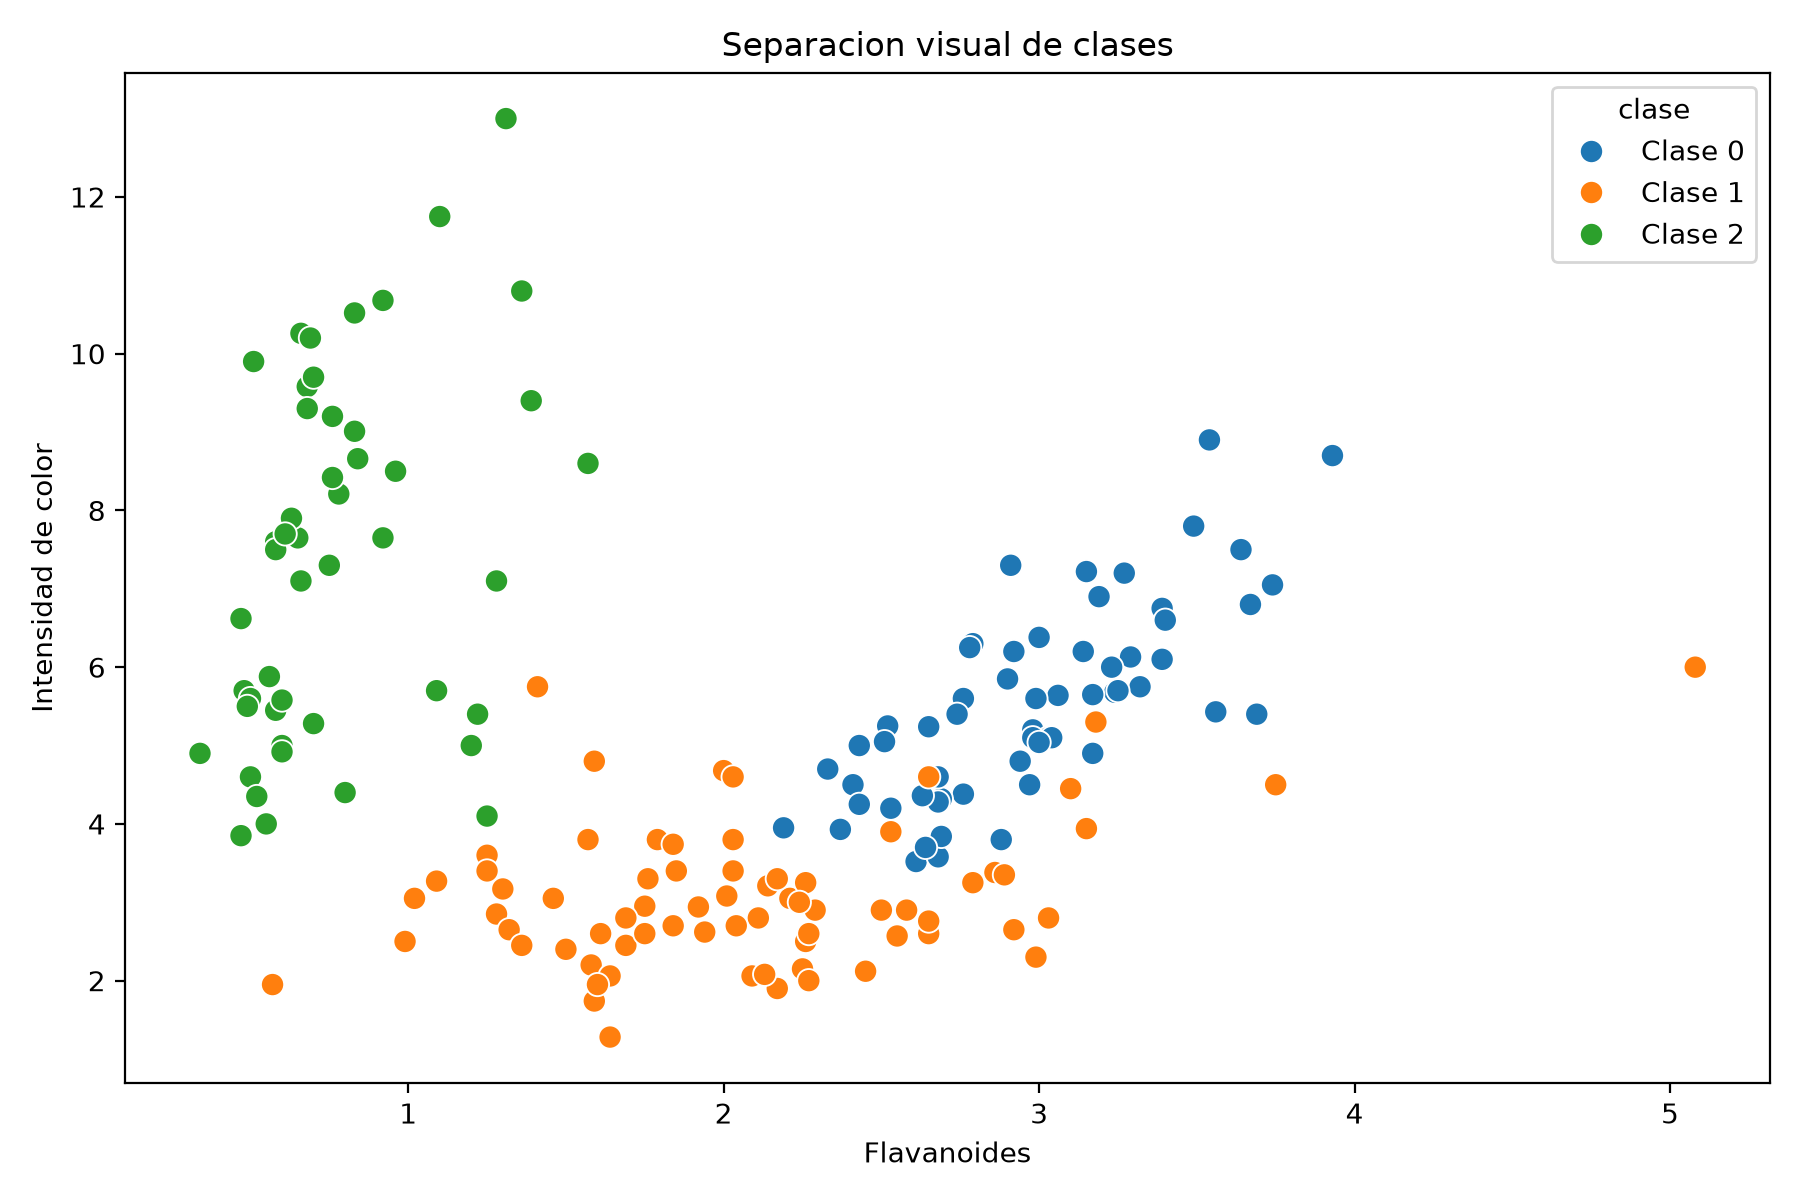
\includegraphics[
width=0.8\textwidth,
height=0.29\textheight,
keepaspectratio
]{dispersion_caracteristicas.png}
\caption{Separación visual de clases mediante
dos características químicas.}
\end{figure}

\subsection{División de datos}

Se aplicó una división estratificada con
\texttt{random\_state=42}:

\begin{itemize}
\item Entrenamiento: 142 observaciones.
\item Prueba: 36 observaciones.
\end{itemize}

El escalado se integró dentro de un Pipeline,
evitando utilizar información del conjunto
de prueba para ajustar las transformaciones.

\subsection{Selección del hiperparámetro}

Se examinaron valores:

\begin{equation}
K \in \{1,2,\ldots,60\}.
\end{equation}

Para cada configuración se utilizó validación
cruzada estratificada de cinco particiones.

El criterio de selección fue:

\begin{equation}
K^* =
\underset{K}{\arg\max}
\left(
\frac{1}{5}
\sum_{i=1}^{5}
\operatorname{Accuracy}_i(K)
\right).
\end{equation}

El conjunto de prueba permaneció reservado
durante la selección del hiperparámetro.

\section{Resultados}

\subsection{Optimización del número de vecinos}

El mejor valor observado fue:

\begin{equation}
\boxed{K^*=29}
\end{equation}

con una exactitud promedio de validación
cruzada de:

\begin{equation}
\overline{\operatorname{Accuracy}}_{\mathrm{CV}}
=0.978818.
\end{equation}

\begin{figure}[H]
\centering
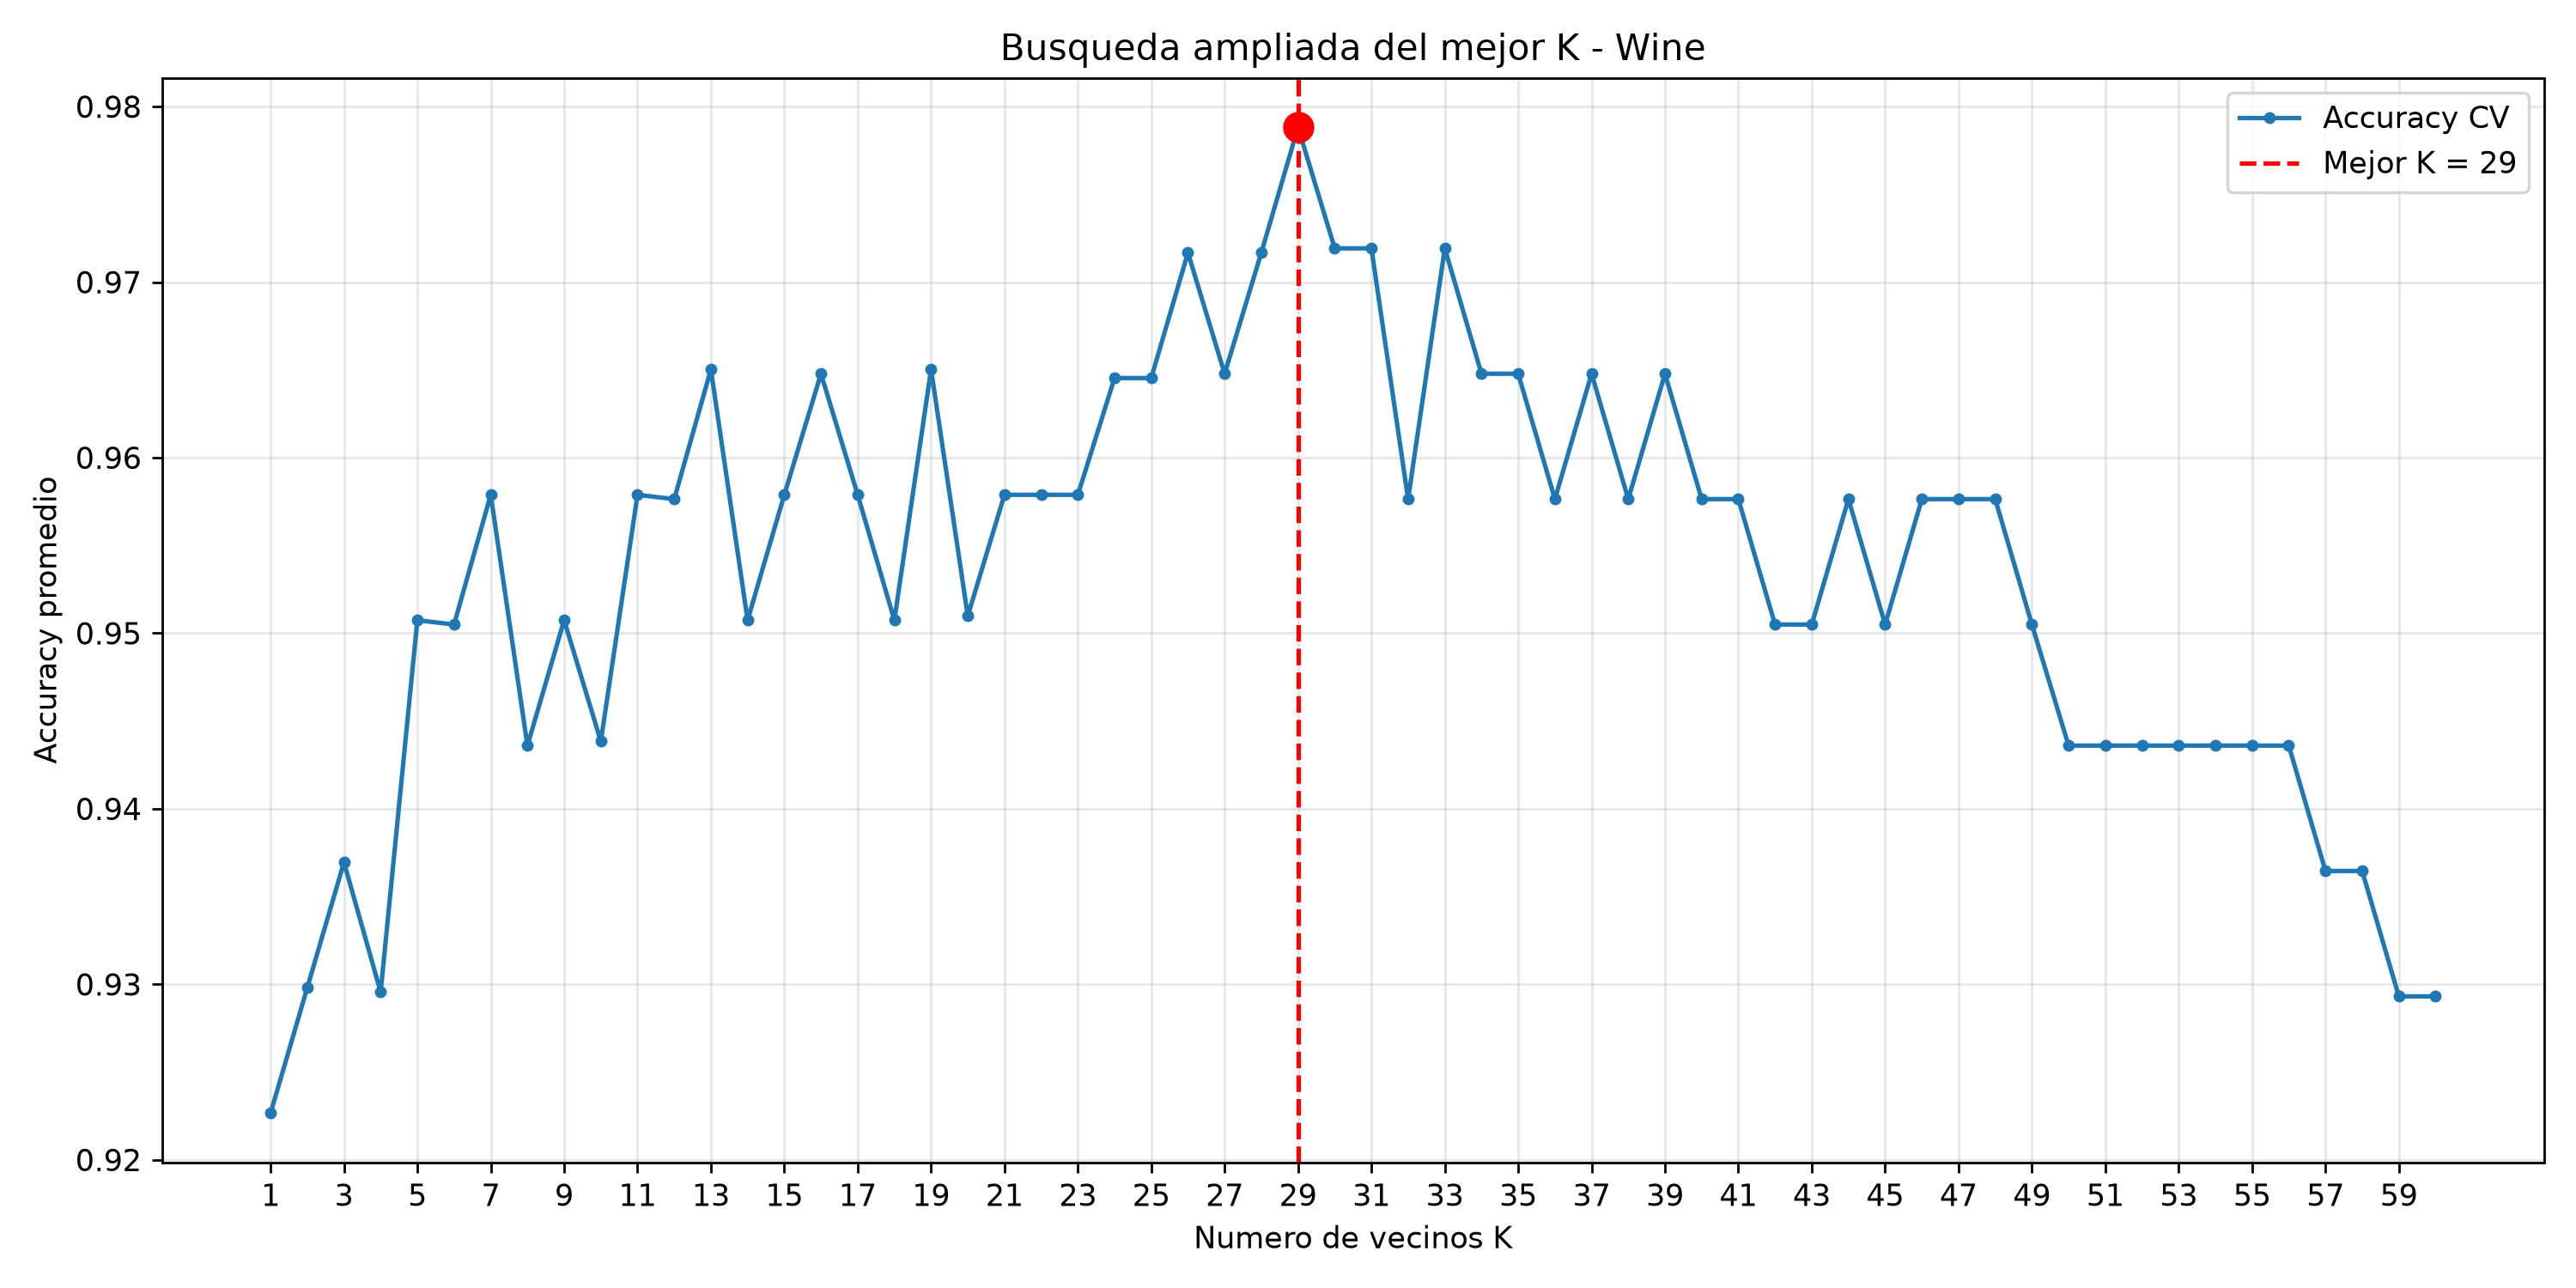
\includegraphics[
width=0.94\textwidth,
height=0.34\textheight,
keepaspectratio
]{optimizacion_k_extendida.png}
\caption{Búsqueda del mejor valor de $K$
en el intervalo de 1 a 60.}
\end{figure}

\subsection{Evaluación final}

El modelo seleccionado se ajustó sobre
las 142 observaciones de entrenamiento
y se evaluó sobre las 36 observaciones
de prueba.

\begin{table}[H]
\centering
\caption{Métricas de evaluación final}
\begin{tabular}{lr}
\toprule
Métrica & Resultado \\
\midrule
Accuracy & 97.22\% \\
Balanced accuracy & 97.62\% \\
Precision macro & 97.44\% \\
Recall macro & 97.62\% \\
F1-score macro & 97.43\% \\
\bottomrule
\end{tabular}
\end{table}

El clasificador acertó 35 observaciones
y cometió un único error.

\subsection{Matriz de confusión}

La matriz de confusión obtenida fue:

\begin{equation}
C=
\begin{pmatrix}
12 & 0 & 0 \\
1 & 13 & 0 \\
0 & 0 & 10
\end{pmatrix}.
\end{equation}

Las filas representan las etiquetas reales
y las columnas las predicciones.

\begin{figure}[H]
\centering
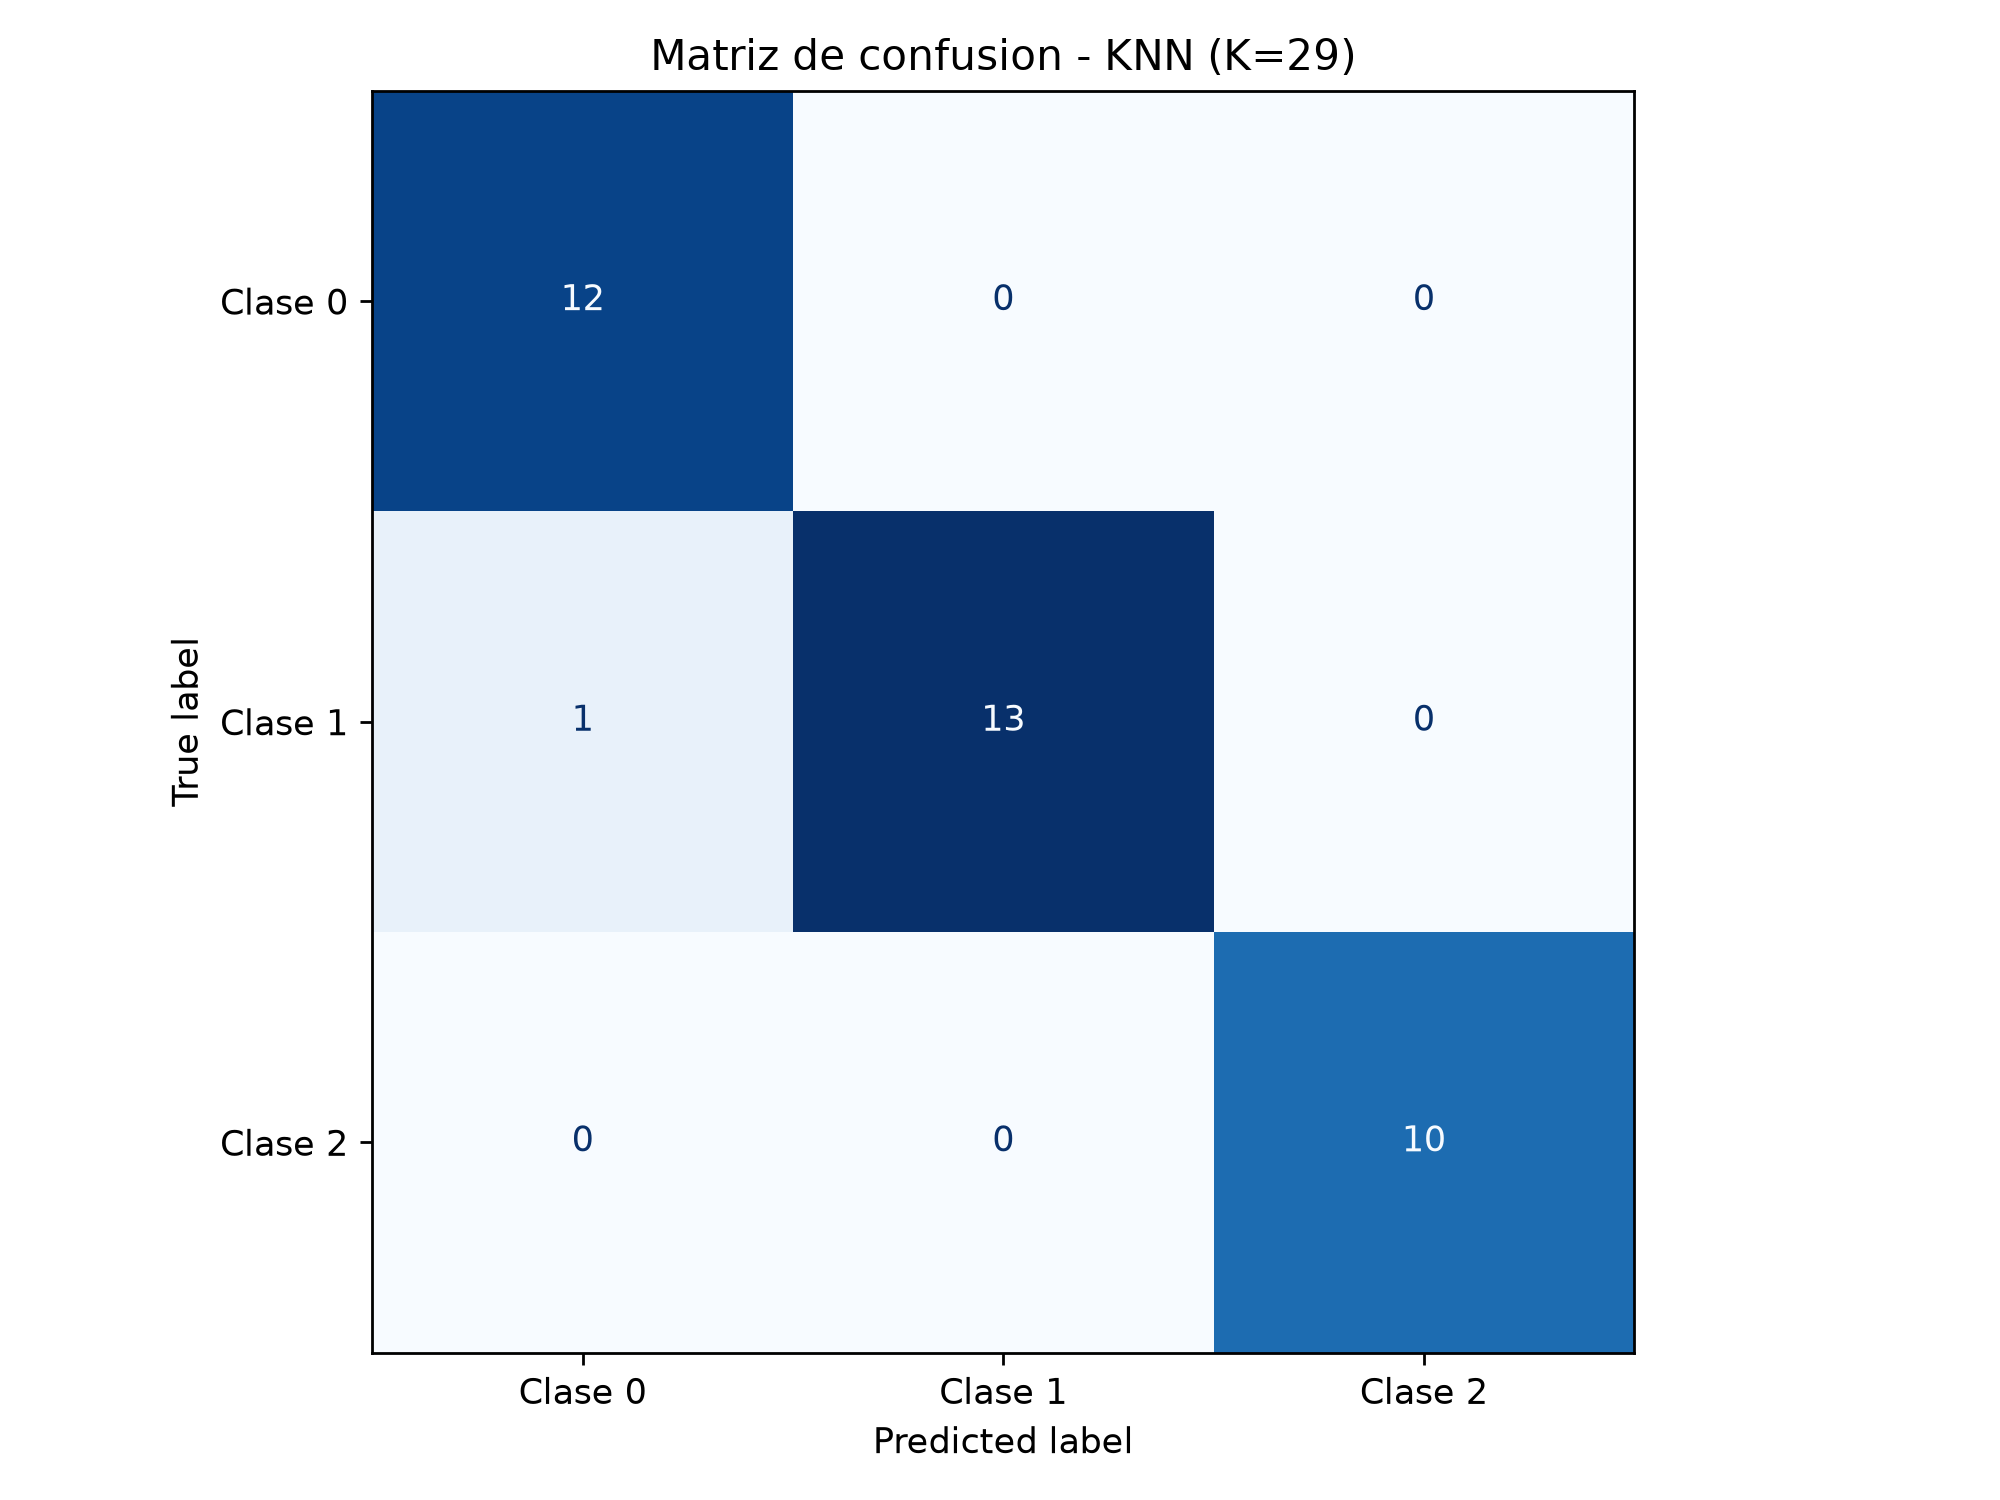
\includegraphics[
width=0.72\textwidth,
height=0.32\textheight,
keepaspectratio
]{matriz_confusion_final.png}
\caption{Matriz de confusión del clasificador
final con $K=29$.}
\end{figure}

El único error corresponde a una
observación de clase 1 clasificada como
clase 0.

\subsection{Predicción demostrativa}

Se utilizó una observación sintética
con trece características químicas.

El modelo predijo la clase 0 y los
29 vecinos seleccionados votaron
por dicha clase.

Este resultado demuestra la capacidad
de inferencia del modelo, pero no
representa una nueva evaluación,
pues la etiqueta real es desconocida.

\section{Discusión}

El valor $K=29$ presentó el mayor accuracy
promedio dentro del conjunto de valores
examinados.

La evaluación final obtuvo una exactitud
de 97.22\%, cercana al resultado de
validación cruzada de 97.88\%.

No obstante, el conjunto de prueba
contiene únicamente 36 observaciones.
Por ello, no puede afirmarse que el
rendimiento observado esté garantizado
sobre nuevas poblaciones de datos.

Además, la diferencia entre varios valores
de $K$ fue pequeña y podría variar con
otras particiones de entrenamiento.

\section{Conclusiones}

El clasificador KNN permitió resolver
satisfactoriamente un problema de
clasificación supervisada multiclase.

La estandarización de las variables
fue metodológicamente importante
debido a sus diferentes escalas.

La validación cruzada permitió seleccionar
$K=29$ sin utilizar el conjunto de prueba
para optimizar el hiperparámetro.

El desempeño final fue de 35 aciertos
sobre 36 observaciones, equivalente
a un accuracy de 97.22\%.

Se recomienda ampliar la evaluación
en trabajos futuros con particiones
adicionales y conjuntos independientes.

\begin{thebibliography}{9}

\bibitem{uci}
UCI Machine Learning Repository.
\textit{Wine Dataset}.
\url{https://archive.ics.uci.edu/dataset/109/wine}.

\bibitem{sklearn}
Scikit-learn.
\textit{Wine Recognition Dataset}.
\url{https://scikit-learn.org/stable/modules/generated/sklearn.datasets.load_wine.html}.

\bibitem{knn}
Scikit-learn.
\textit{KNeighborsClassifier}.
\url{https://scikit-learn.org/stable/modules/generated/sklearn.neighbors.KNeighborsClassifier.html}.

\end{thebibliography}

\end{document}
